
%\documentstyle[epsf,twocolumn]{jarticle}       %LaTeX2e仕様
% \documentclass[twocolumn]{jarticle}     %pLaTeX2e仕様(platex.exeの場合)
\documentclass[onecolumn]{ujarticle}   %pLaTeX2e仕様(uplatex.exeの場合)
%%%%%%%%%%%%%%%%%%%%%%%%%%%%%%%%%%%%%%%%%%%%%%%%%%%%%%%%%%%%%%
%%
%%  基本バージョン
%%
%%%%%%%%%%%%%%%%%%%%%%%%%%%%%%%%%%%%%%%%%%%%%%%%%%%%%%%%%%%%%%%%
\setlength{\topmargin}{-45pt}
%\setlength{\oddsidemargin}{0cm}
\setlength{\oddsidemargin}{-7.5mm}
%\setlength{\evensidemargin}{0cm}
\setlength{\textheight}{24.1cm}
%setlength{\textheight}{25cm}
\setlength{\textwidth}{17.4cm}
%\setlength{\textwidth}{172mm}
\setlength{\columnsep}{11mm}

%\kanjiskip=.07zw plus.5pt minus.5pt


% 【節が変わるごとに (1.1)(1.2) … (2.1)(2.2) と数式番号をつけるとき】
%\makeatletter
%\renewcommand{\theequation}{%
%\thesection.\arabic{equation}} %\@addtoreset{equation}{section}
%\makeatother

%\renewcommand{\arraystretch}{0.95} 行間の設定
%%%%%%%%%%%%%%%%%%%%%%%%%%%%%%%%%%%%%%%%%%%%%%%%%%%%%%%%
%\usepackage{graphicx}   %pLaTeX2e仕様(\documentstyle ->\documentclass)
\usepackage[dvipdfmx]{graphicx}
\usepackage{subcaption}
\usepackage{multirow}
\usepackage{amsmath}
\usepackage{url}
\usepackage{ulem}
\usepackage{algorithm}
\usepackage{algorithmic}
\usepackage{listings} %,jlisting} %日本語のコメントアウトをする場合jlistingが必要
%ここからソースコードの表示に関する設定
\lstset{
  basicstyle={\ttfamily},
  identifierstyle={\small},
  commentstyle={\smallitshape},
  keywordstyle={\small\bfseries},
  ndkeywordstyle={\small},
  stringstyle={\small\ttfamily},
  frame={tb},
  breaklines=true,
  columns=[l]{fullflexible},
  numbers=left,
  xrightmargin=0zw,
  xleftmargin=3zw,
  numberstyle={\scriptsize},
  stepnumber=1,
  numbersep=1zw,
  lineskip=-0.5ex
}
\newcommand{\argmax}{\mathop{\rm arg~max}\limits}
\newcommand{\argmin}{\mathop{\rm arg~min}\limits}

%%%%%%%%%%%%%%%%%%%%%%%%%%%%%%%%%%%%%%%%%%%%%%%%%%%%%%%%
\begin{document}

	%bibtex用の設定
	%\bibliographystyle{ujarticle}

	% \twocolumn[
		\noindent
		\hspace{1em}
		2022 年 9 月 2 日
		ゼミ資料
		\hfill
		杉山 竜弥
		\vspace{2mm}

		\hrule
		\begin{center}
			{\Large \bf 進捗報告}
		\end{center}
		\hrule
		\vspace{9mm}
	% ]


\section{今週やったこと}
\begin{itemize}
  \item データセット準備
\end{itemize}


\section{データセット準備}
Video ViT を使用しようとしていたが,
現在整備している画像データだと
データ長不足(1つのデータが 3 コマしかないものも)やデータの長さが不均一という問題があったため,
このデータをそのまま ViViT に与えるのは難しいと判断した.

そこで Youtube 上の動画から動画データセットを作成する方針と
一旦 ViT に一枚ずつデータを入力する方針に分けて進める.

\subsection{ViT}
事前学習した ViT に自作の画像フォルダを読み込ませるところまでは動作を確認した.
MLP に通す前の特徴ベクトルを獲得すれば,絵描き歌の 1 フレームの情報は取得できる状態になった.

\subsection{動画データセット}
動画をデータセットにする場合を調査した.
Youtube からダウンロードはできたので,
open cv で画像に書き出せばデータセットの読み込みは出来ると思われる.

1データあたりの情報量は増えるが,グラデーションがかかっていたり歌詞の字幕ついていたりアスペクト比がばらばらだったりするので,ノイズは画像よりも多い.

\section{予定}
\begin{itemize}
  \item 実験方針を決める
\end{itemize}


% \begin{figure}[h]
%   \begin{center}
%     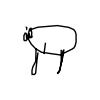
\includegraphics[clip,width=20mm]{decode1.png}
%     \caption{比較元のデコードスケッチ}
%     \label{fig:result2_1}
%   \end{center}
% \end{figure}

% 参考文献リスト
% \bibliographystyle{unsrt}
% \bibliography{ref}
\end{document}
